%%%%%%%%%%%%%%%%%%%%%%%%%%%%%%%%%%%%%%%%%%%%%%%%%%%%
\section{Confronto del modello di coalescenza e di PYTHIA}
Sebbene non nella sua configurazione predefinita, \pythiaa{} ammette anche la produzione deuteronica tramite il modello di coalescenza.
Per far ciò si è andati a ridurre l'insieme di tutti i possibili canali di produzione al singolo canale della cattura radiativa (l'unico rilevante per la coalescenza), assegnando ad essa il modello di coalescenza con il parametro $p_0 = 195$ MeV.
La scelta di questo valore è giustificata da una semplice valutazione della \autoref{tab:valori_p0_1sigma0}: andando ad osservare la colonna $p_0$ si può dedurre che esso raggiunge stabilmente questo valore già a 7 TeV.
Dopodiché, oltre a questo, si è andati a imporre le condizioni già riportate nella \autoref{ch:settings} e si è effettuata la simulazione di Monte Carlo.\\

Andando a osservare lo spettro di produzione di $p+\bar p$ (visibile in \autoref{fig:E_pp}), non si nota una particolare differenza col modello predefinito, come deve essere, dal momento in cui il numero di (anti)deuteroni prodotti dovrebbe essere relativamente piccolo rispetto a quello dei protoni sia per il modello di \pythiaa{} sia per il modello di coalescenza.
\begin{figure}[htb]
    \centering
    \begin{subfigure}{.49\textwidth}
    \centering
        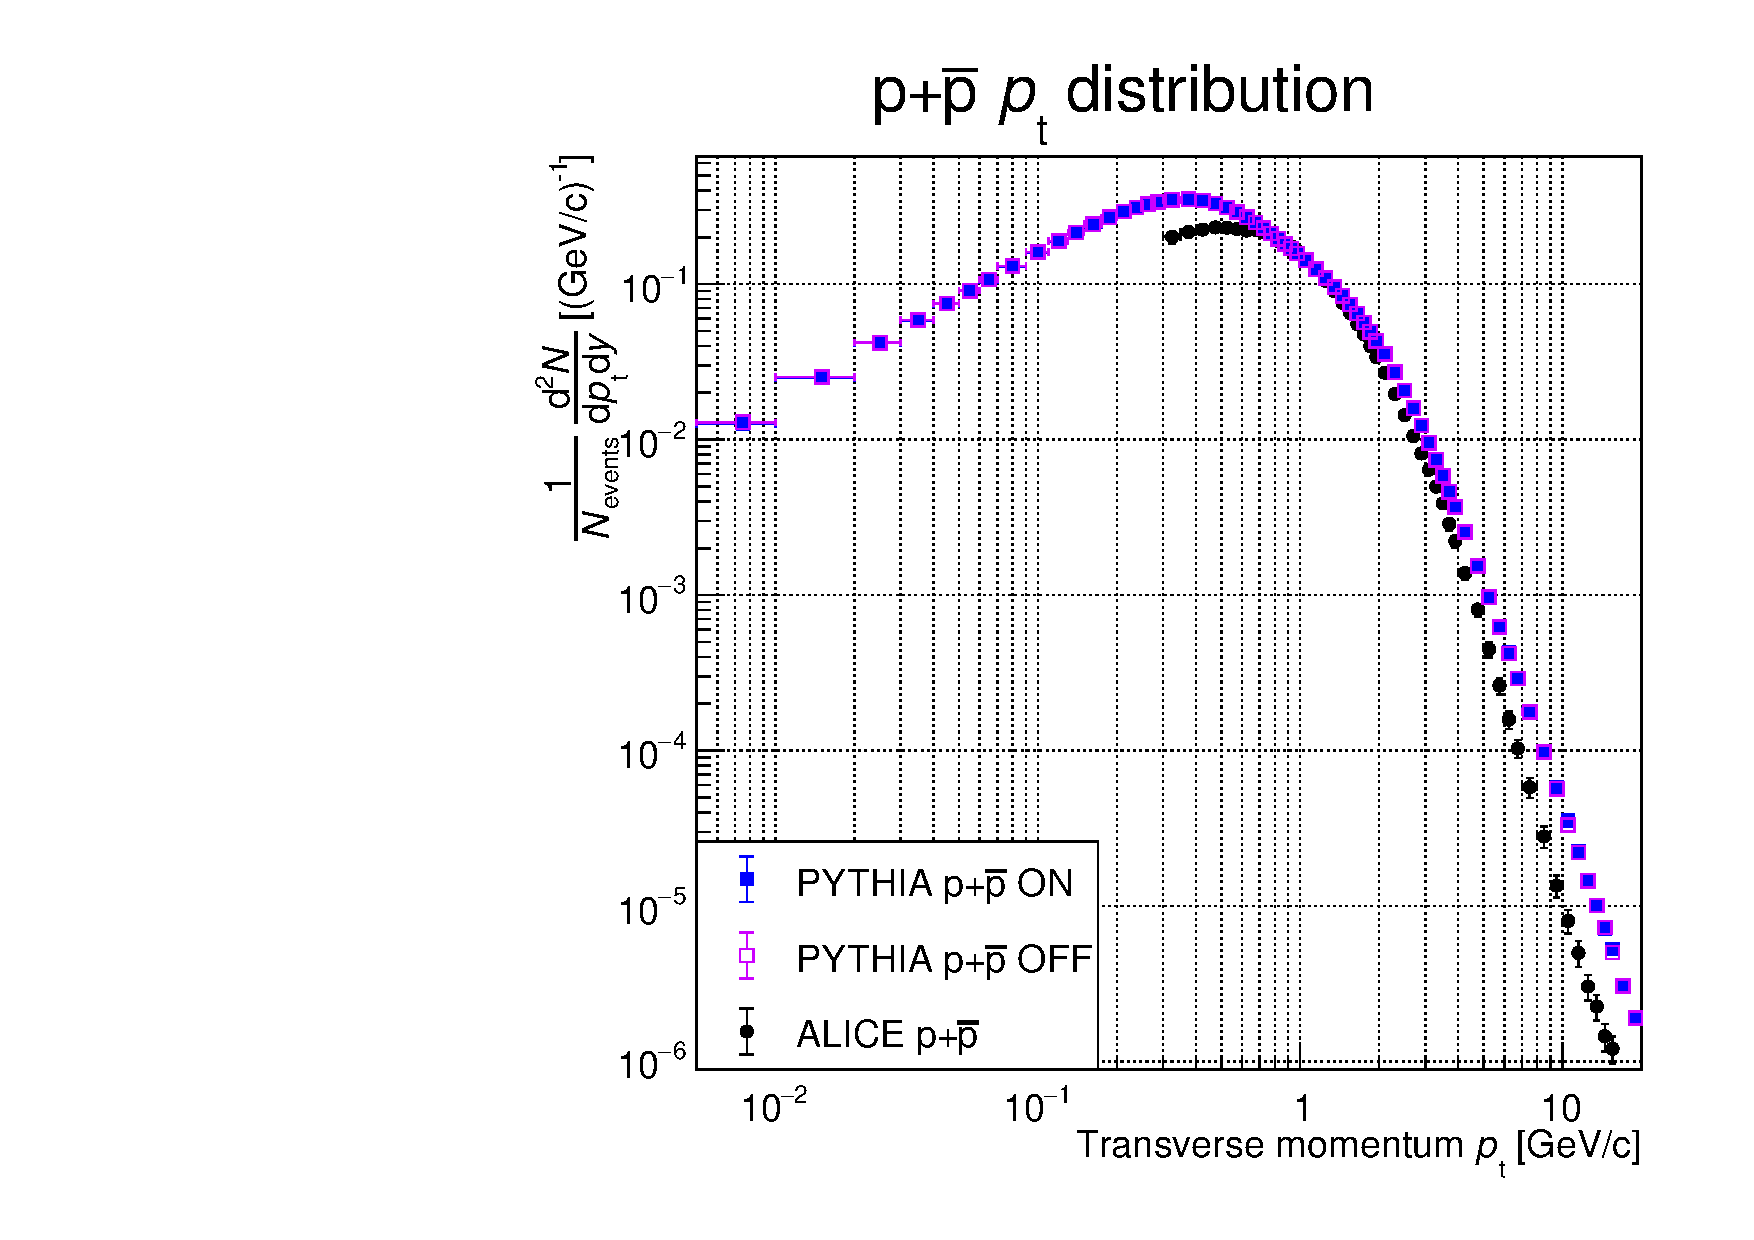
\includegraphics[width=\textwidth]{image/3-risultati/analyse/E/pp.pdf}
        \caption{}
        \label{fig:E_pp}
    \end{subfigure}
    %\hspace{1cm}
    \begin{subfigure}{.49\textwidth}
        \centering
        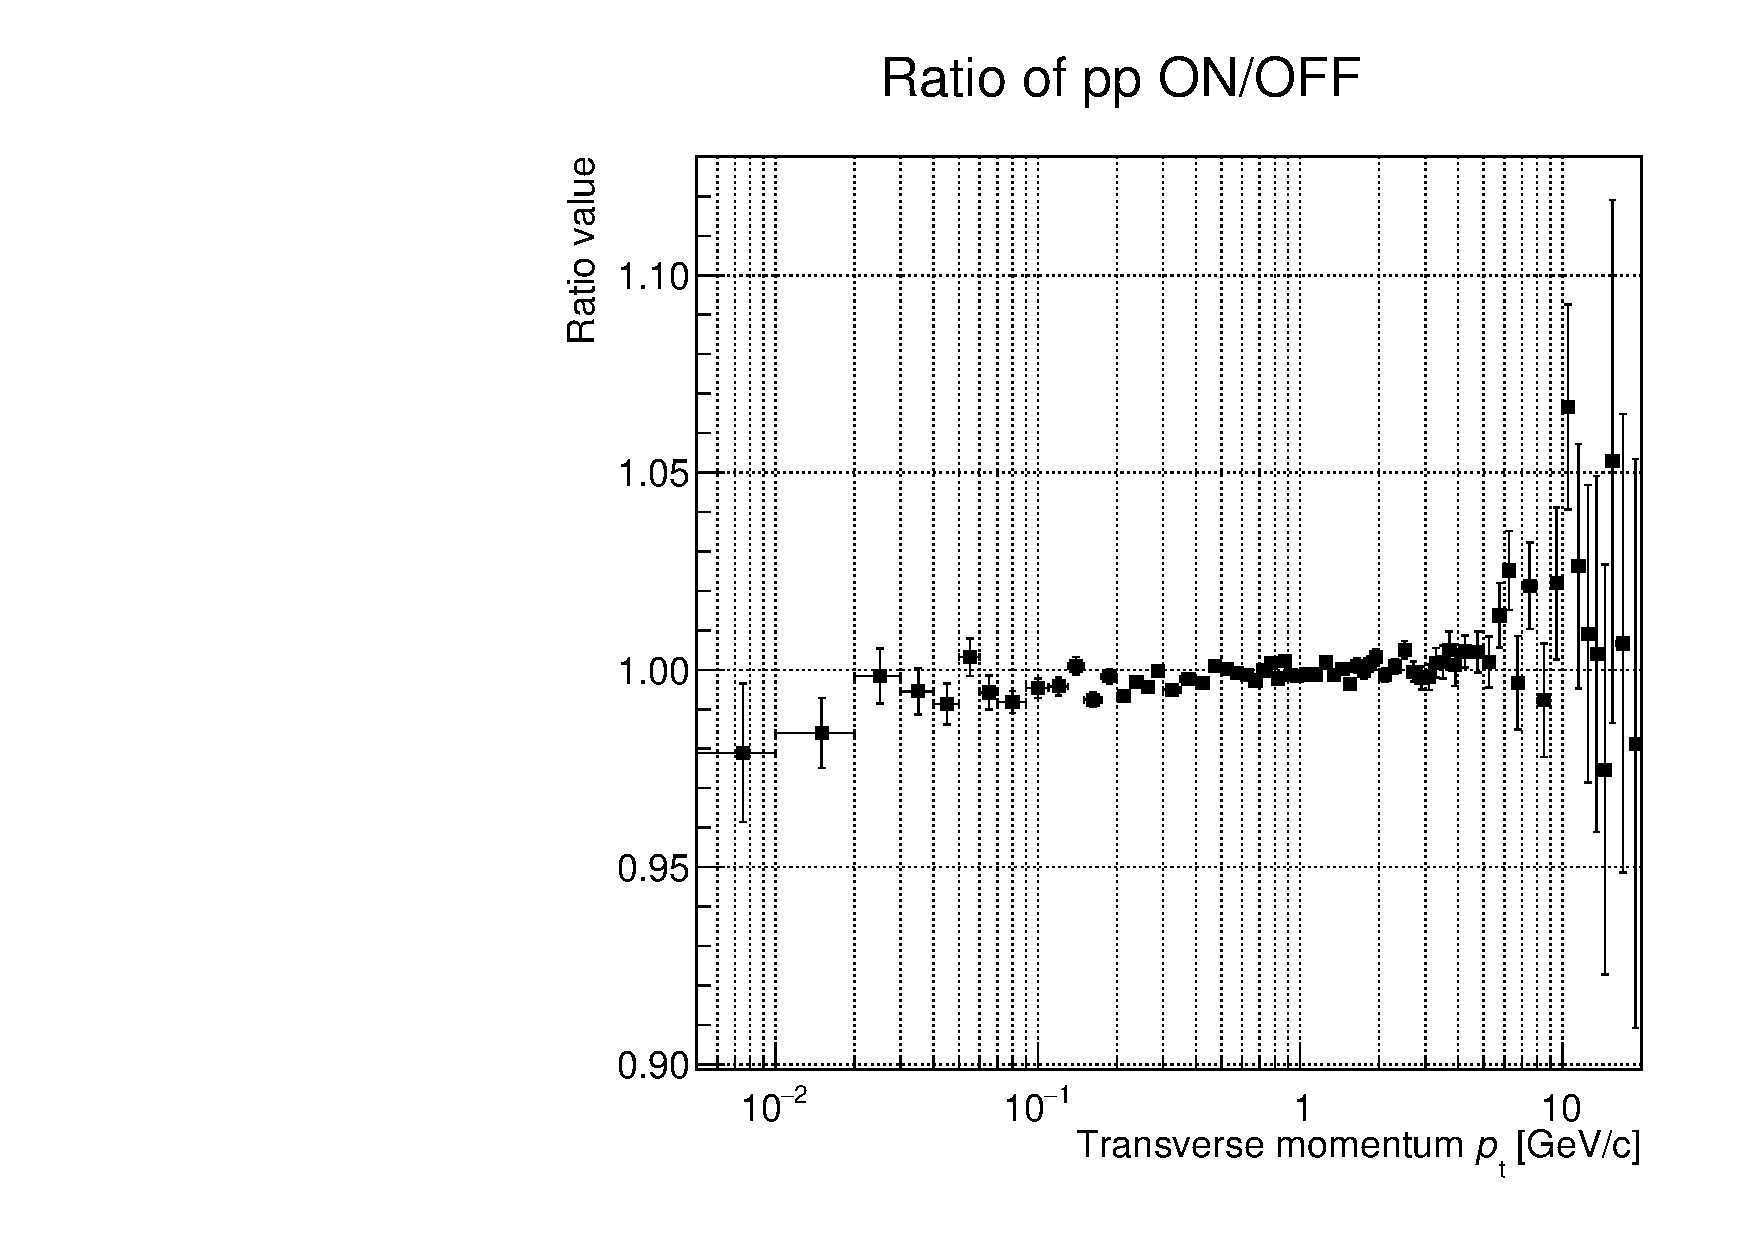
\includegraphics[width=\textwidth]{image/3-risultati/analyse/E/ratio_pp_ON_OFF.pdf}
        \caption{}
        \label{fig:E_ratio_pp_ON_OFF}
    \end{subfigure}
    \captionwithsource{\emph{\rmfamily (a)} Distribuzione dell'impulso trasverso di $p+\bar p$ con produzione deuteronica attivata e disattivata ("ON" e "OFF") in confronto con i dati sperimentali di ALICE ("ALICE"), usando il modello di coalescenza. \emph{\rmfamily (b)} Frazione della distribuzione dell'impulso trasverso di $p+\bar p$ con produzione deuteronica attivata e con produzione non attivata, usando il modello di coalescenza.}{\cite{ALICE:2020jsh}}
    \label{fig:E_pp_prod}
\end{figure}
Neanche la divisione tra il caso in cui la produzione deuteronica sia attivata e quella disattivata presenta particolari differenze, come si può notare in \autoref{fig:E_ratio_pp_ON_OFF}, con un valore della media pesata di $0.99873 \pm 0.00023$, vicino al valore di 0.999.

Invece gli spettri di produzione dei (anti)deuteroni (\autoref{fig:E_(anti)deuteron}) hanno un andamento diverso, come deve essere, visto che i diversi modelli utilizzati sono differenti.
Da questi grafici si osserva un andamento discordante degli spettri per tutto il dominio dei dati di ALICE, sottolineando l'inadeguatezza del modello di coalescenza. 
Eseguendo una divisione tra i dati dei (anti)deuteroni di \pythia{} e di ALICE otteniamo il grafico riportato in \autoref{fig:E_division} ed eseguendo una media pesata del rapporto otteniamo il valore di $0.793 \pm 0.012$ per i deuteroni e $0.738 \pm 0.016$ per gli antideuteroni, quindi una sottoproduzione di circa 20-30\%.\\

Come verifica ulteriore della correttezza delle predizioni è stato misurato il rapporto tra gli istogrammi dei deuteroni e degli antideuteroni (\autoref{fig:E_ratio_DD}), ottenendo un valore della media pesata di $1.008 \pm 0.008$, compatibile con il valore unitario.\\

Ora, eseguendo invece una divisione tra il modello di coalescenza e il modello predefinito di \pythiaa{}, si ottiene il grafico visibile in \autoref{fig:A_vs_E}.
I due modelli presentano un andamento simile solamente nel range tra $0.1-1$ GeV/$c$, in cui per entrambi si è osservato una sovrapproduzione di (anti)deuteroni rispetto ai dati di ALICE.
\begin{figure}[htbp]
    \centering
    \begin{subfigure}{.49\textwidth}
    \centering
        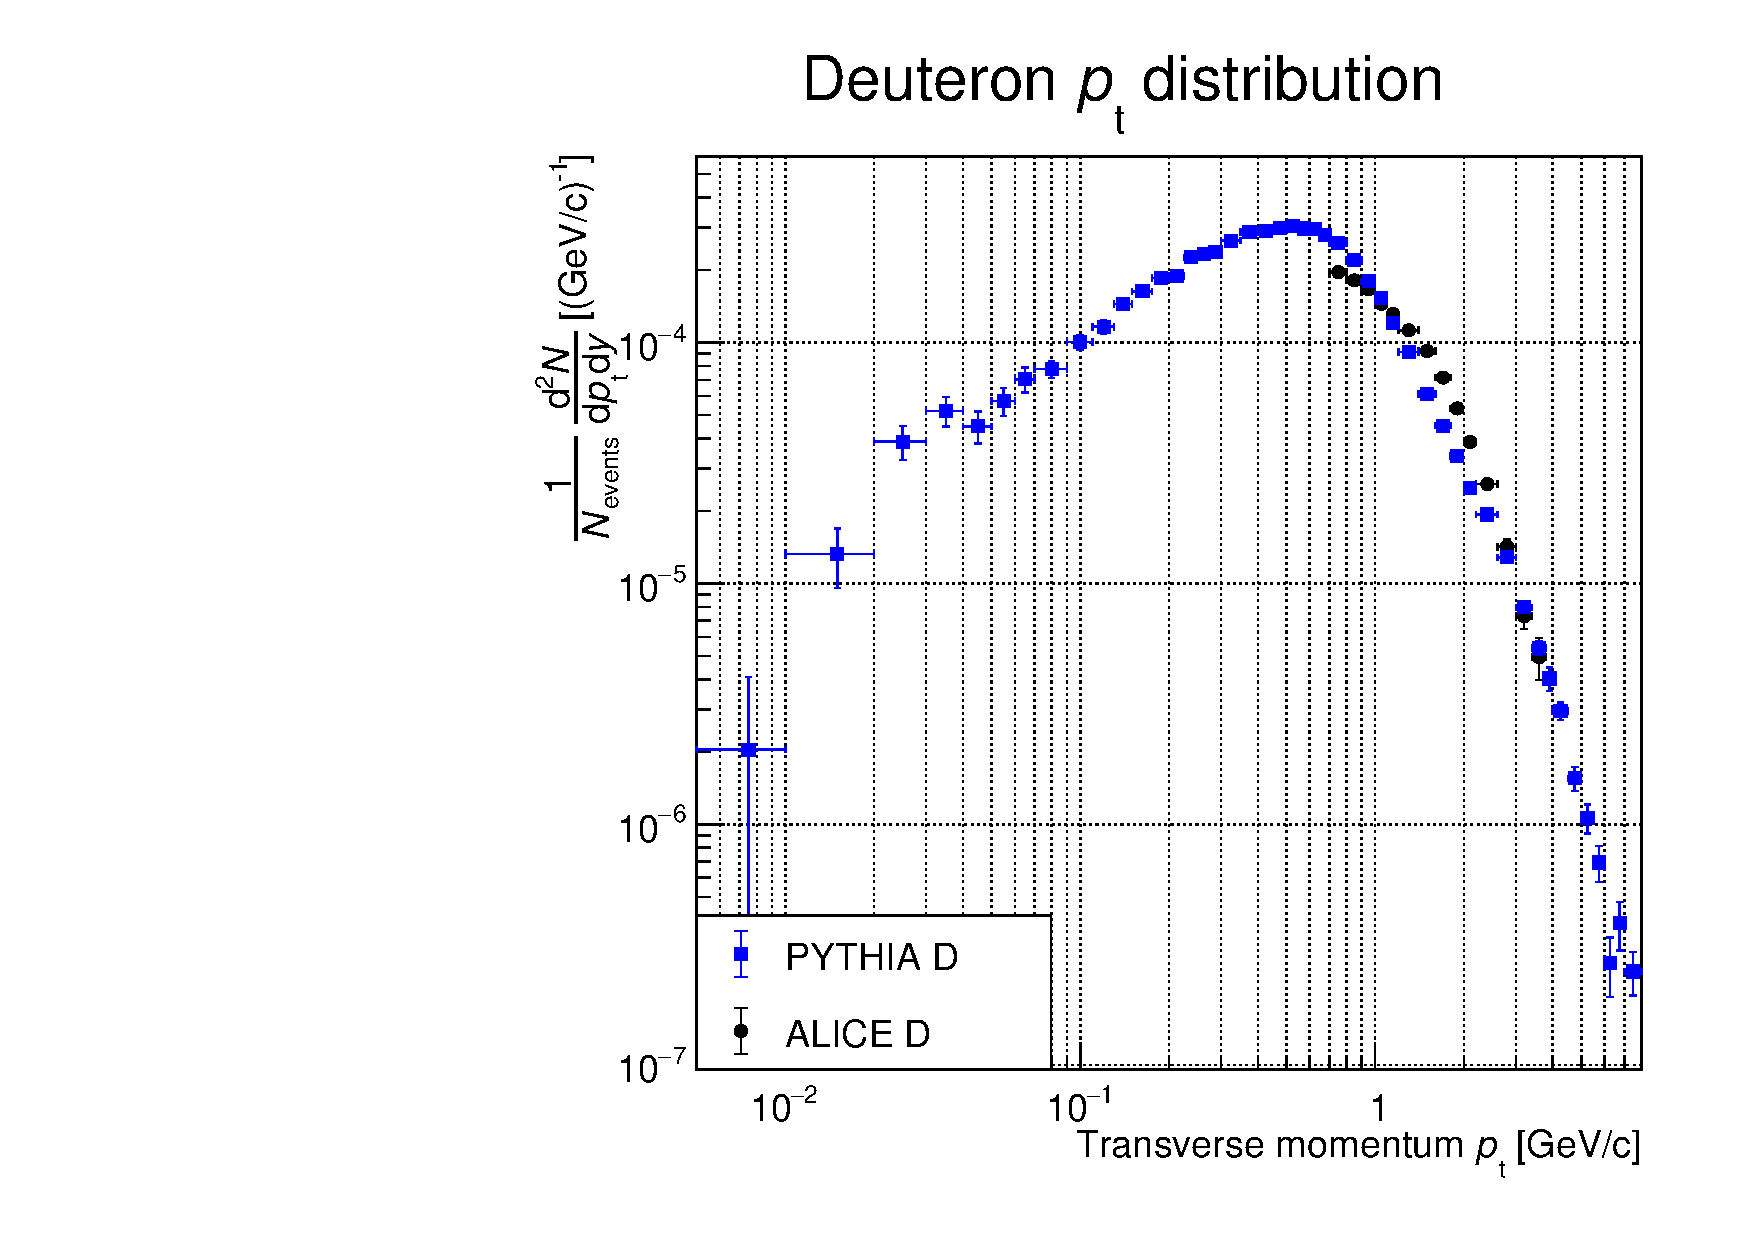
\includegraphics[width=\textwidth]{image/3-risultati/analyse/E/deuteron.pdf}
        \caption{}
        \label{fig:E_deuteron}
    \end{subfigure}
    %\hspace{1cm}
    \begin{subfigure}{.49\textwidth}
        \centering
        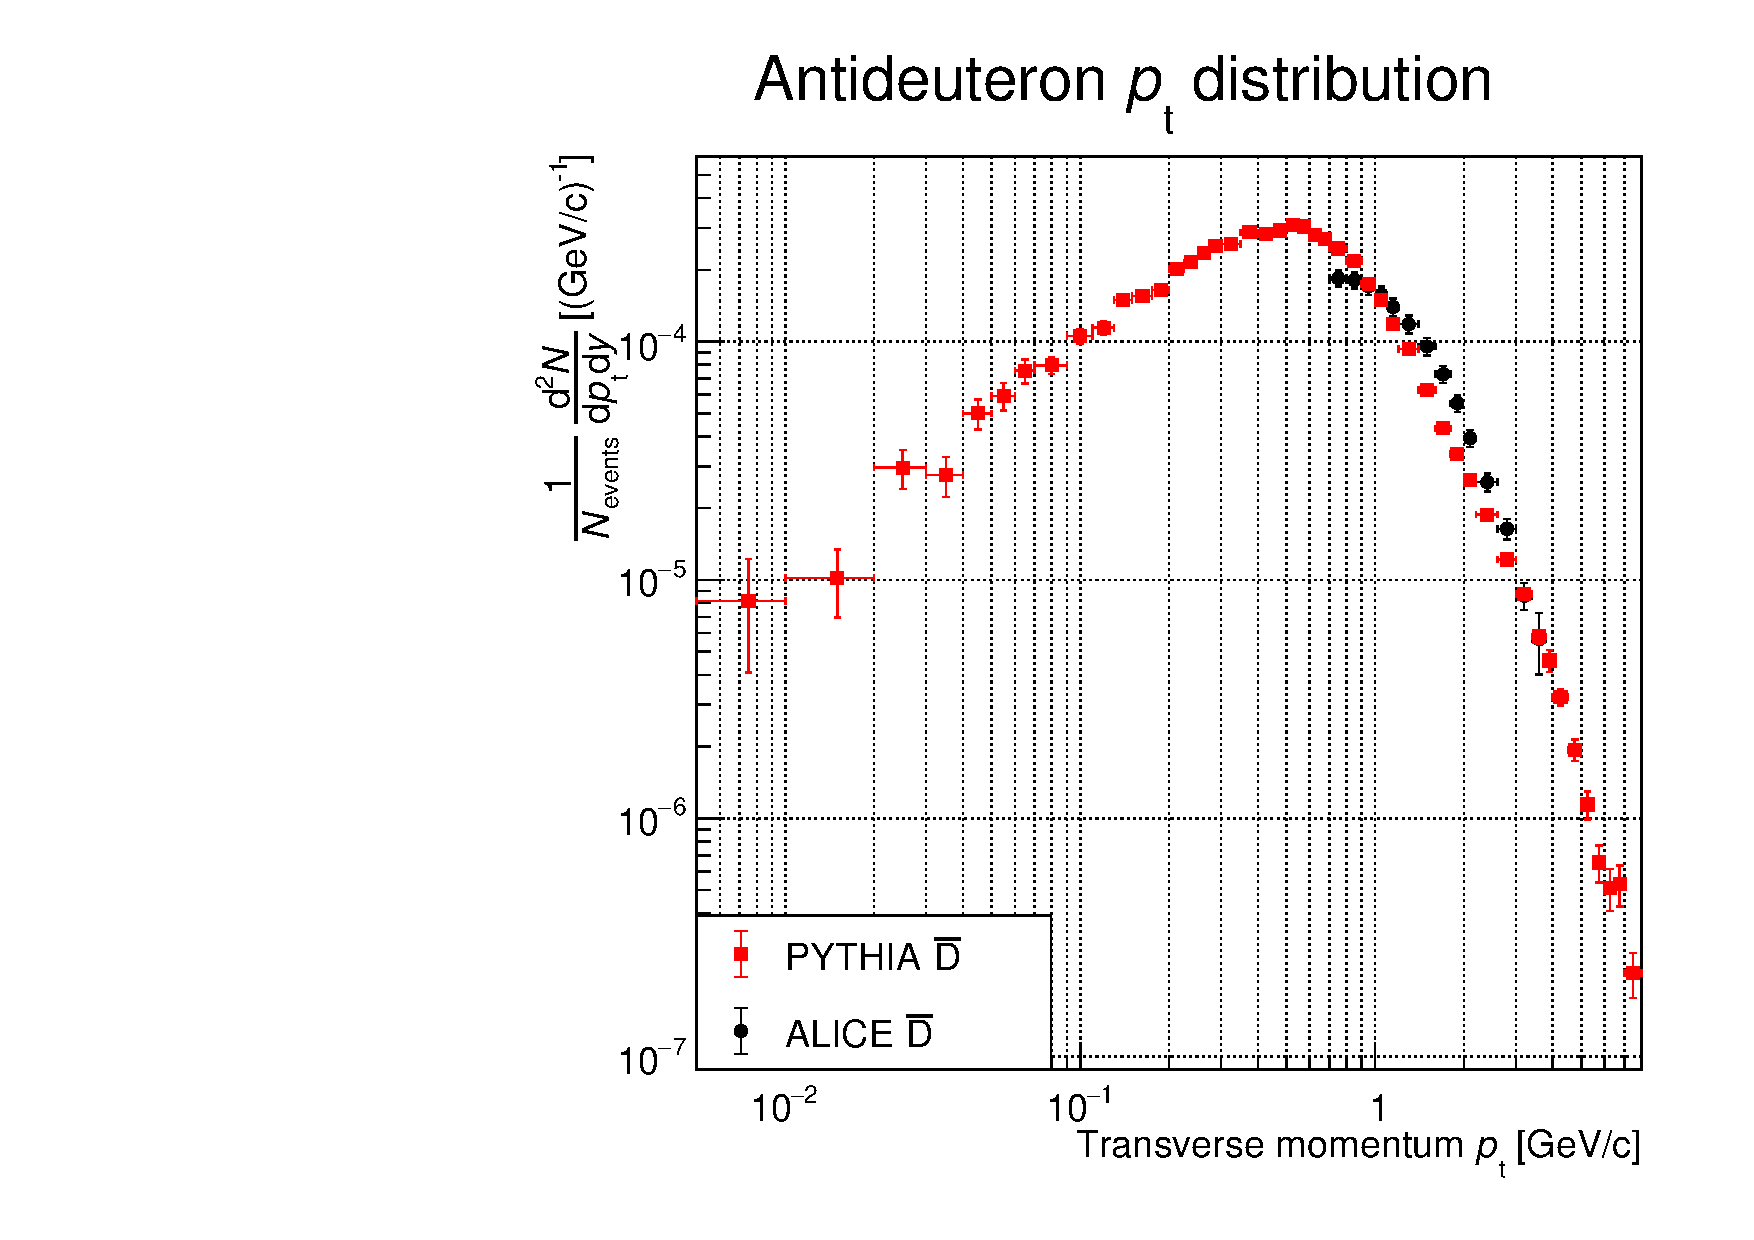
\includegraphics[width=\textwidth]{image/3-risultati/analyse/E/antideuteron.pdf}
        \caption{}
        \label{fig:E_antideuteron}
    \end{subfigure}
    \captionwithsource{Distribuzione dell'impulso trasverso di \emph{\rmfamily (a)} $D$ e \emph{\rmfamily (b)} di $\bar D$ in confronto con i dati di ALICE, utilizzando il modello di coalescenza.}{\cite{ALICE:2020foi}}
    \label{fig:E_(anti)deuteron}
\end{figure}
\begin{figure}[htbp]
    \centering
    \begin{subfigure}{.49\textwidth}
    \centering
        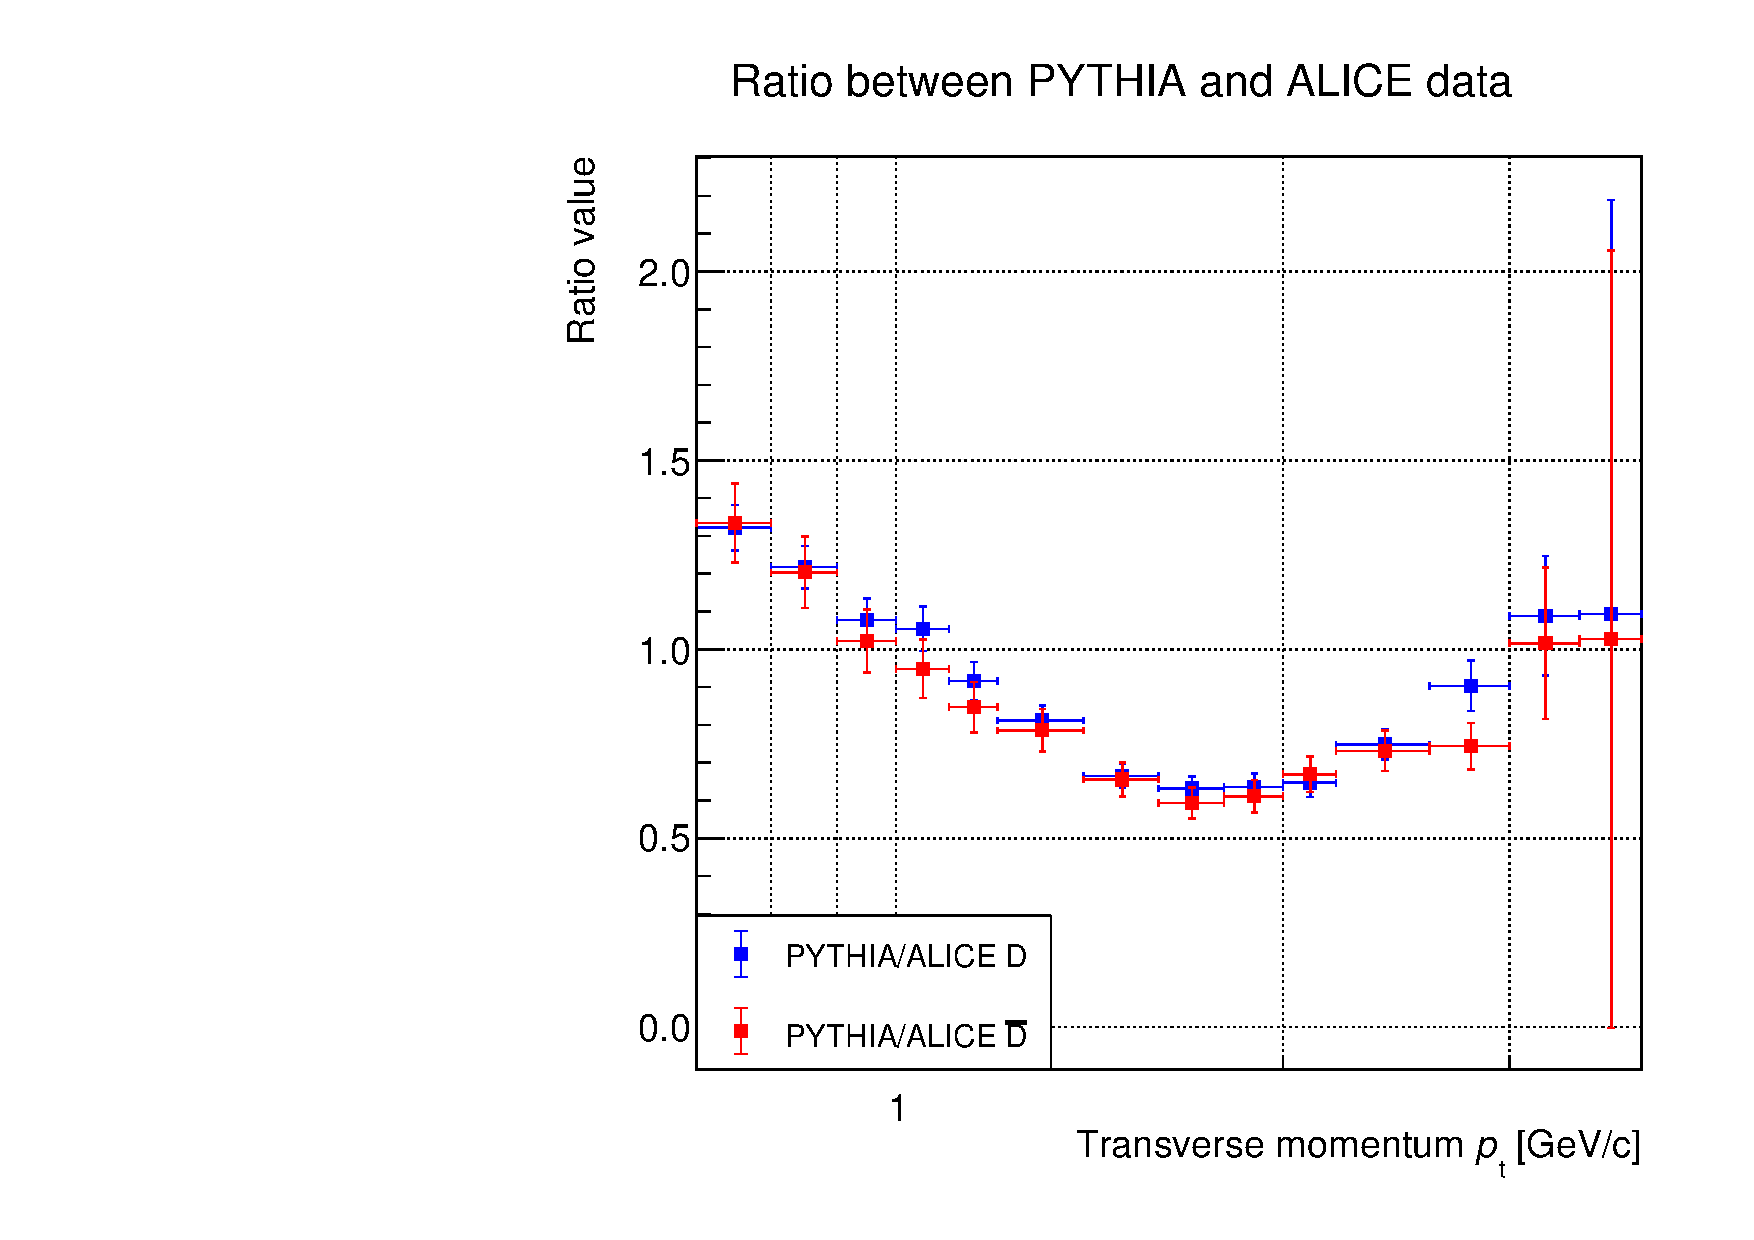
\includegraphics[width=\textwidth]{image/3-risultati/analyse/E/division.pdf}
        \caption{}
        \label{fig:E_division}
    \end{subfigure}
    %\hspace{1cm}
    \begin{subfigure}{.49\textwidth}
        \centering
        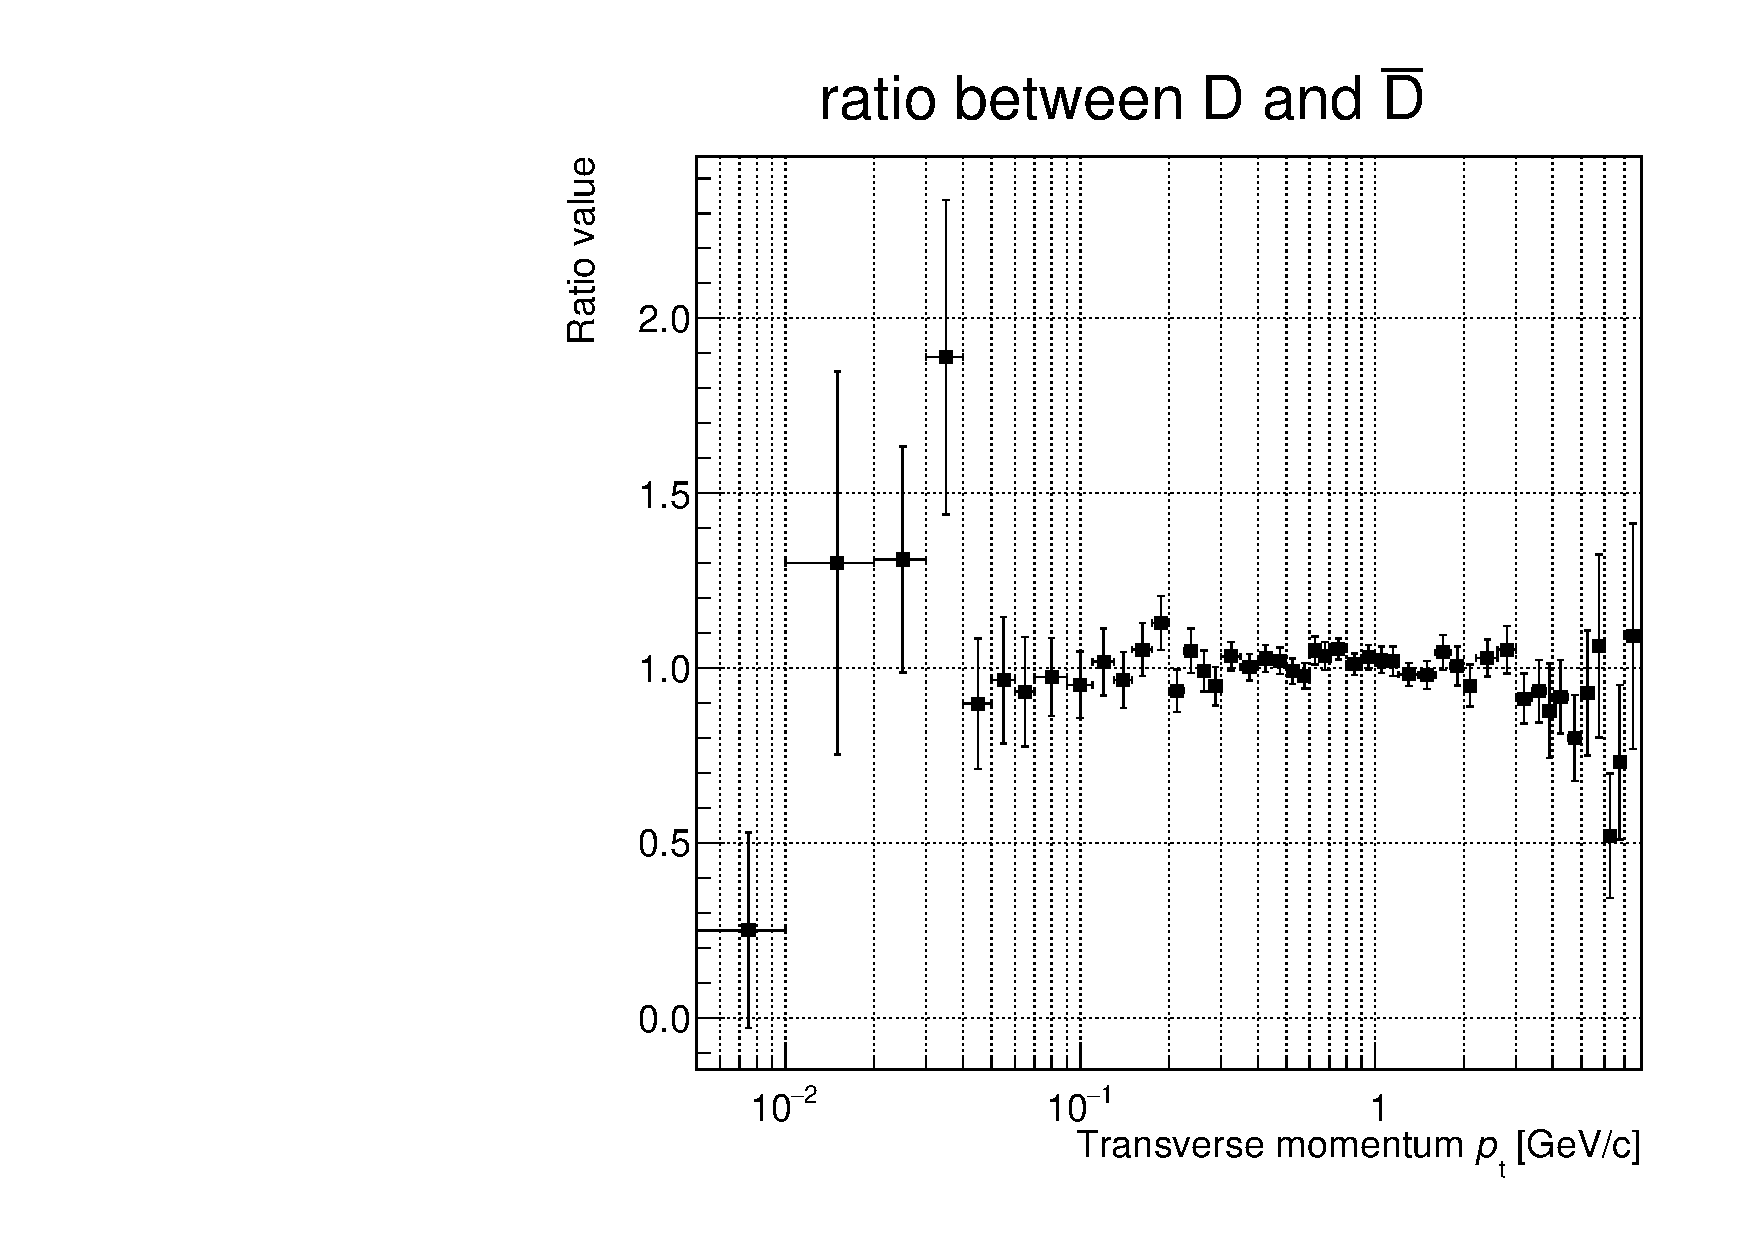
\includegraphics[width=\textwidth]{image/3-risultati/analyse/E/ratio_DD.pdf}
        \caption{}
        \label{fig:E_ratio_DD}
    \end{subfigure}
    \caption{\emph{\rmfamily (a)} Divisione tra la distribuzione dell'impulso trasverso di $D$ e $\bar D$ con i dati di ALICE, utilizzando il modello di coalescenza. \emph{\rmfamily (b)} Frazione delle distribuzione dell'impulso trasverso di $D$ con quello di $\bar D$, utilizzando il modello di coalescenza.}
    \label{fig:E_ratio_DD_}
\end{figure}
\begin{figure}[htp]
    \centering
    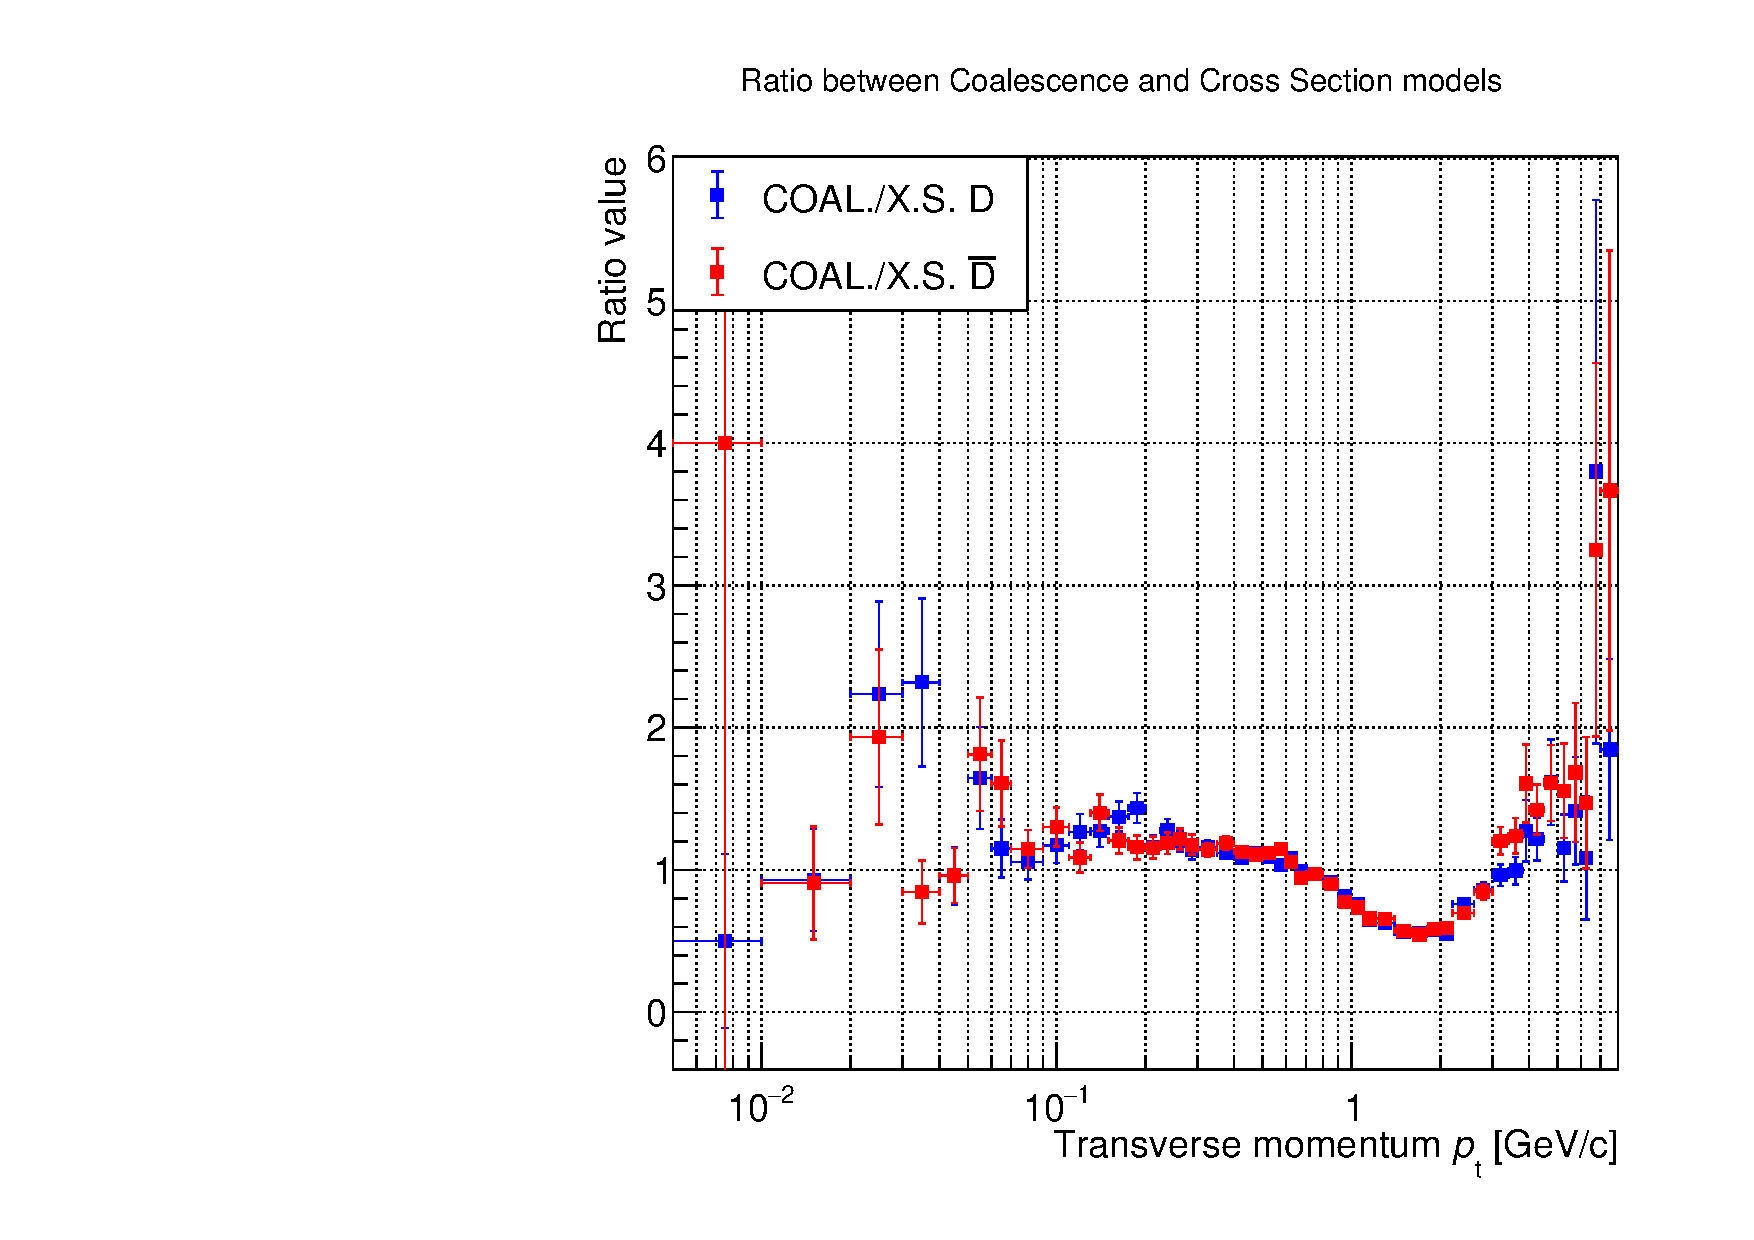
\includegraphics[width=0.49\textwidth]{image/3-risultati/analyse/A/ratio_CXS.pdf}
    \caption{Rapporto tra la distribuzione dell'impulso trasverso di $D$ e $\bar D$ ottenuta con il modello di coalescenza e con il modello predefinito di \emph{\pythiaa}. "COAL" indica il modello di coalescenza, "X.S." indica il modello di \pythiaa{}.}
    \label{fig:A_vs_E}
\end{figure}